
有些对象没有特定的长度。要想知道长度,需要遍历它们的所有元素。例如,在本章的其他地方,我们已经看到了一个没有特定长度的生成器,更常见的例子是C字串。

C-string是由字符组成的C数组,以空值“\verb|\|0”作为结束。

\hspace*{\fill} \\ %插入空行
\begin{center}
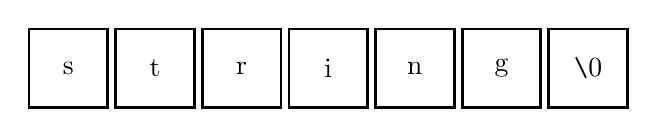
\begin{tikzpicture}
\draw[line width=1pt] (1.1*0,1) rectangle (1.1*0+1,0) node[pos=.5] {s};
\draw[line width=1pt] (1.1*1,1) rectangle (1.1*1+1,0) node[pos=.5] {t};
\draw[line width=1pt] (1.1*2,1) rectangle (1.1*2+1,0) node[pos=.5] {r};
\draw[line width=1pt] (1.1*3,1) rectangle (1.1*3+1,0) node[pos=.5] {i};
\draw[line width=1pt] (1.1*4,1) rectangle (1.1*4+1,0) node[pos=.5] {n};
\draw[line width=1pt] (1.1*5,1) rectangle (1.1*5+1,0) node[pos=.5] {g};
\draw[line width=1pt] (1.1*6,1) rectangle (1.1*6+1,0) node[pos=.5] {\verb|\|0};
\end{tikzpicture}

图4.5 带有空结束符的C-string
\end{center}

即使没有意识到,我们也一直在使用C-string。C/C++中的字面值字符串都是C-string:

\begin{lstlisting}[style=styleCXX]
std::string s = "string";
\end{lstlisting}

这里,STL字符串s初始化为一个字面值字符串。字面值字符串是一个C字串。若看一下十六进制中的单个字符,就会看到结束符:

\begin{lstlisting}[style=styleCXX]
for (char c : "string") {
	std::cout << format("{:02x} ", c);
}
\end{lstlisting}

单词“string”有六个字母。循环的输出显示了数组中的七个元素:

\begin{tcblisting}{commandshell={}}
73 74 72 69 6e 67 00
\end{tcblisting}

第7个是空——结束符。

循环看到的是包含7个值的C字符数组,是一个字符串的事实对循环是不可见的抽象。若想让循环像对待字符串一样对待它,需要一个迭代器和一个哨兵。

哨兵是一个对象,标志着一个长度不确定的迭代器的结束。当迭代器到达数据的末尾时,哨兵将与迭代器进行相等比较。

为了了解这是如何工作的,先为C-string构建一个迭代器!

\subsubsection{How to do it…}

要使用带有C-string哨兵,需要构建一个自定义迭代器。不需要很复杂,只需要使用基于范围的for循环的基本要素即可。

\begin{itemize}
\item 
先从几个定义开始:

\begin{lstlisting}[style=styleCXX]
using sentinel_t = const char;
constexpr sentinel_t nullchar = '\0';
\end{lstlisting}

sentinel\_t是const char的别名,我们的哨兵就用这个类型。

我们还为空字符结束符定义了常量nullchar。

\item 
现在来定义迭代器类型:

\begin{lstlisting}[style=styleCXX]
class cstr_it {
	const char *s{};
public:
	explicit cstr_it(const char *str) : s{str} {}
	char operator*() const { return *s; }
	cstr_it& operator++() {
		++s;
		return *this;
	}
	bool operator!=(sentinel_t) const {
		return s != nullptr && *s != nullchar;
	}
	cstr_it begin() const { return *this; }
	sentinel_t end() const { return nullchar; }
};
\end{lstlisting}

这是基于范围的for循环所必需的最小值,end()函数返回一个nullchar,操作符!=()重载与nullchar进行比较。这就是哨兵所需要的。

\item 
现在,可以定义一个函数,使用哨兵来打印C-string:

\begin{lstlisting}[style=styleCXX]
void print_cstr(const char * s) {
	cout << format("{}: ", s);
	for (char c : cstr_it(s)) {
		std::cout << format("{:02x} ", c);
	}
	std::cout << '\n';
}
\end{lstlisting}

这个函数中,首先打印字符串。然后,使用format()函数将每个字符打印为十六进制值。

\item 
现在,可以在main()中调用print\_cstr():

\begin{lstlisting}[style=styleCXX]
int main() {
	const char carray[]{"array"};
	print_cstr(carray);
	const char * cstr{"c-string"};
	print_cstr(cstr);
}
\end{lstlisting}

输出如下所示:

\begin{tcblisting}{commandshell={}}
array: 61 72 72 61 79
c-string: 63 2d 73 74 72 69 6e 67
\end{tcblisting}

注意,这里没有多余的字符,也没有空终止符。因为哨兵告诉for循环,在看到nullchar时停止。

\end{itemize}

\subsubsection{How it works…}

迭代器类的哨兵非常简单,可以通过在end()函数中返回空结束符,将其作为哨兵使用:

\begin{lstlisting}[style=styleCXX]
sentinel_t end() const { return nullchar; }
\end{lstlisting}

然后,可以用不等于比较操作符进行测试:

\begin{lstlisting}[style=styleCXX]
bool operator!=(sentinel_t) const {
	return s != nullptr && *s != nullchar;
}
\end{lstlisting}


注意,参数只是一个类型(sentinel\_t)。参数类型是函数签名必需的,但我们不需要值,要做的就是将当前迭代器与哨兵进行比较。

当类型或类没有预定的比较终点时,就会使用这种方法。



















